\documentclass[11pt,a4paper]{article}

% LuaLaTeX Greek support
\usepackage{fontspec}
\usepackage{polyglossia}
\setmainlanguage{greek}
\setotherlanguage{english}

% Fonts - Using standard system fonts that usually support Greek
\newfontfamily\greekfont[Script=Greek]{FreeSerif}
\newfontfamily\greekfontsf[Script=Greek]{FreeSans}

\usepackage{amsmath}
\usepackage{amssymb}
\usepackage{graphicx}
\usepackage{hyperref}
\usepackage{geometry}
\usepackage{listings}
\usepackage{xcolor}

\geometry{margin=1in}

\title{Artificial Intelligence Project 2 - Phase A Report}
\author{Ομάδα Εργασίας}
\date{\today}

\begin{document}

\maketitle

\section{Εισαγωγή}
Η παρούσα αναφορά περιγράφει την υλοποίηση και σύγκριση τριών πρακτόρων τοπικής αναζήτησης σε μη-στατικά περιβάλλοντα: \textbf{Hill Climbing}, \textbf{Random Restart Hill Climbing} και \textbf{Simulated Annealing}. Η αξιολόγηση έγινε στα περιβάλλοντα \texttt{CartPole-v1} και \texttt{MountainCar-v0} της βιβλιοθήκης \texttt{ns-gym}, τα οποία χαρακτηρίζονται από μεταβαλλόμενες φυσικές παραμέτρους.

\section{Υλοποίηση Wrappers (\texttt{wrappers/wrappers.py})}
Οι wrappers υλοποιήθηκαν για να τροποποιήσουν την ανταμοιβή και να επιτρέψουν τον σχεδιασμό (planning) μέσω προσομοίωσης.

\subsection{ForwardWrapper και Δυναμικές Παράμετροι}
Η κλάση \texttt{ForwardWrapper} επιτρέπει στους πράκτορες να έχουν πρόσβαση στις μεταβαλλόμενες παραμέτρους του \texttt{ns-gym} (όπως η βαρύτητα και η μάζα). Η μέθοδος \texttt{\_\_getattr\_\_} εξασφαλίζει ότι οι κλήσεις προωθούνται στο εσωτερικό περιβάλλον χωρίς να χάνεται η πληροφορία της μη-στατικότητας.

\subsection{Reward Shaping}
Στη μέθοδο \texttt{step()}, προστίθεται τυχαίος θόρυβος $r_{noisy} = r_{orig} + \epsilon$, καθιστώντας την εκμάθηση πιο απαιτητική. Επιπλέον, η μέθοδος \texttt{reward(action)} παρέχει μια γρήγορη εκτίμηση της επόμενης κατάστασης για lookahead planning.

\section{Πράκτορες Τοπικής Αναζήτησης}

\subsection{Hill Climbing (HC)}
Ο πράκτορας \texttt{HillClimbingAgent} ακολουθεί μια άπληστη (greedy) στρατηγική. Σε κάθε βήμα, αξιολογεί όλες τις δυνατές κινήσεις χρησιμοποιώντας lookahead και επιλέγει αυτή που μεγιστοποιεί την άμεση αναμενόμενη αξία (value). Αν και αποτελεσματικός, ο αλγόριθμος είναι ευάλωτος σε τοπικά μέγιστα.

\subsection{Random Restart Hill Climbing (RRHC)}
Για την αντιμετώπιση των τοπικών μεγίστων, ο \texttt{RandomRestartHillClimbingAgent} εκτελεί πολλαπλές αναζητήσεις Hill Climbing ξεκινώντας από διαφορετικά τυχαία σημεία (ή τυχαίες αρχικές κινήσεις). Στο πλαίσιο της εργασίας, αυτό υλοποιείται μέσω επαναλαμβανόμενων rollouts ή αυξημένης δειγματοληψίας υποψήφιων διαδρομών.

\subsection{Simulated Annealing (SA)}
Ο πράκτορας \texttt{SimulatedAnnealingAgent} επιτρέπει την αποδοχή χειρότερων κινήσεων με πιθανότητα $P = e^{\Delta V / T}$. Αυτό βοηθά στην "απόδραση" από τοπικά μέγιστα, ειδικά στην αρχή του επεισοδίου όπου η θερμοκρασία $T$ είναι υψηλή.

\section{Ευρετικές Συναρτήσεις (Heuristics)}
Η επιτυχία των αλγορίθμων βασίζεται σε ισχυρές ευρετικές συναρτήσεις:
\begin{itemize}
    \item \textbf{CartPole:} $V = 10.0 - (10.0 \cdot \theta^2 + 0.1 \cdot x^2 + 0.5 \cdot \dot{\theta}^2)$, δίνοντας έμφαση στη σταθερότητα της γωνίας και της ταχύτητας.
    \item \textbf{MountainCar:} $V = \text{pos} + 15.0 \cdot \text{vel}^2$, ενθαρρύνοντας την αύξηση της κινητικής ενέργειας για την ανάβαση.
\end{itemize}

\section{Πειραματικά Αποτελέσματα}
Τα αποτελέσματα των πειραμάτων αποτυπώνονται στις παρακάτω γραφικές παραστάσεις.

\subsection{Πείραμα 1: Μέση Ανταμοιβή ανά Timesteps}
Συγκρίνουμε τους πράκτορες για $max\_timesteps \in \{10, 100, 500, 1000\}$.

\begin{figure}[h]
    \centering
    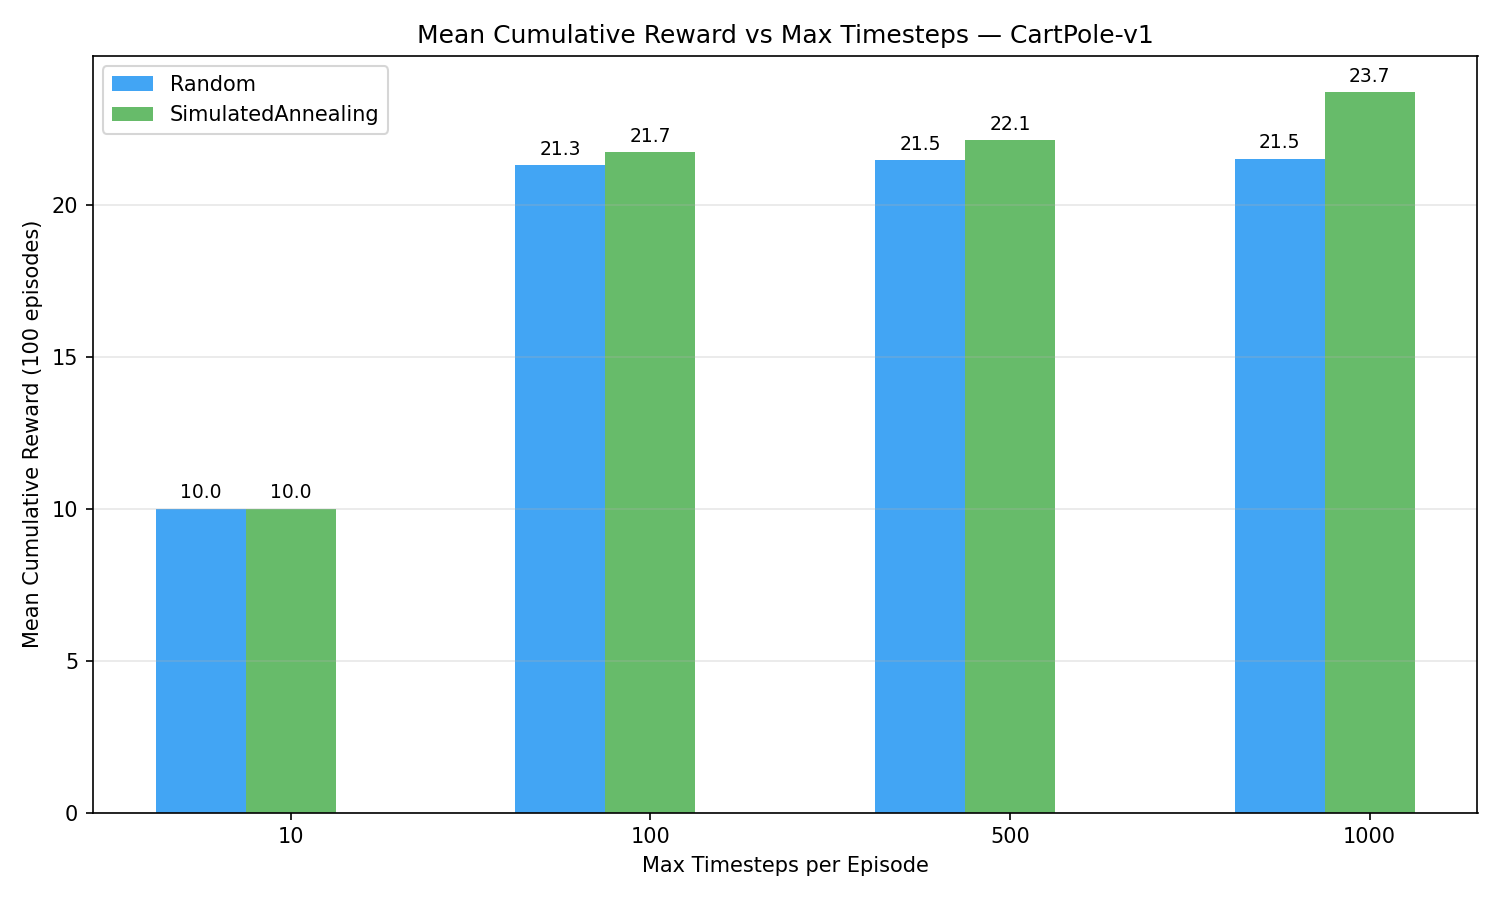
\includegraphics[width=0.85\textwidth]{exp1_CartPole_v1.png}
    \caption{Μέση ανταμοιβή (100 επεισόδια) για το CartPole-v1. Συγκρίνονται οι Random, HC, RRHC και SA.}
\end{figure}

\begin{figure}[h]
    \centering
    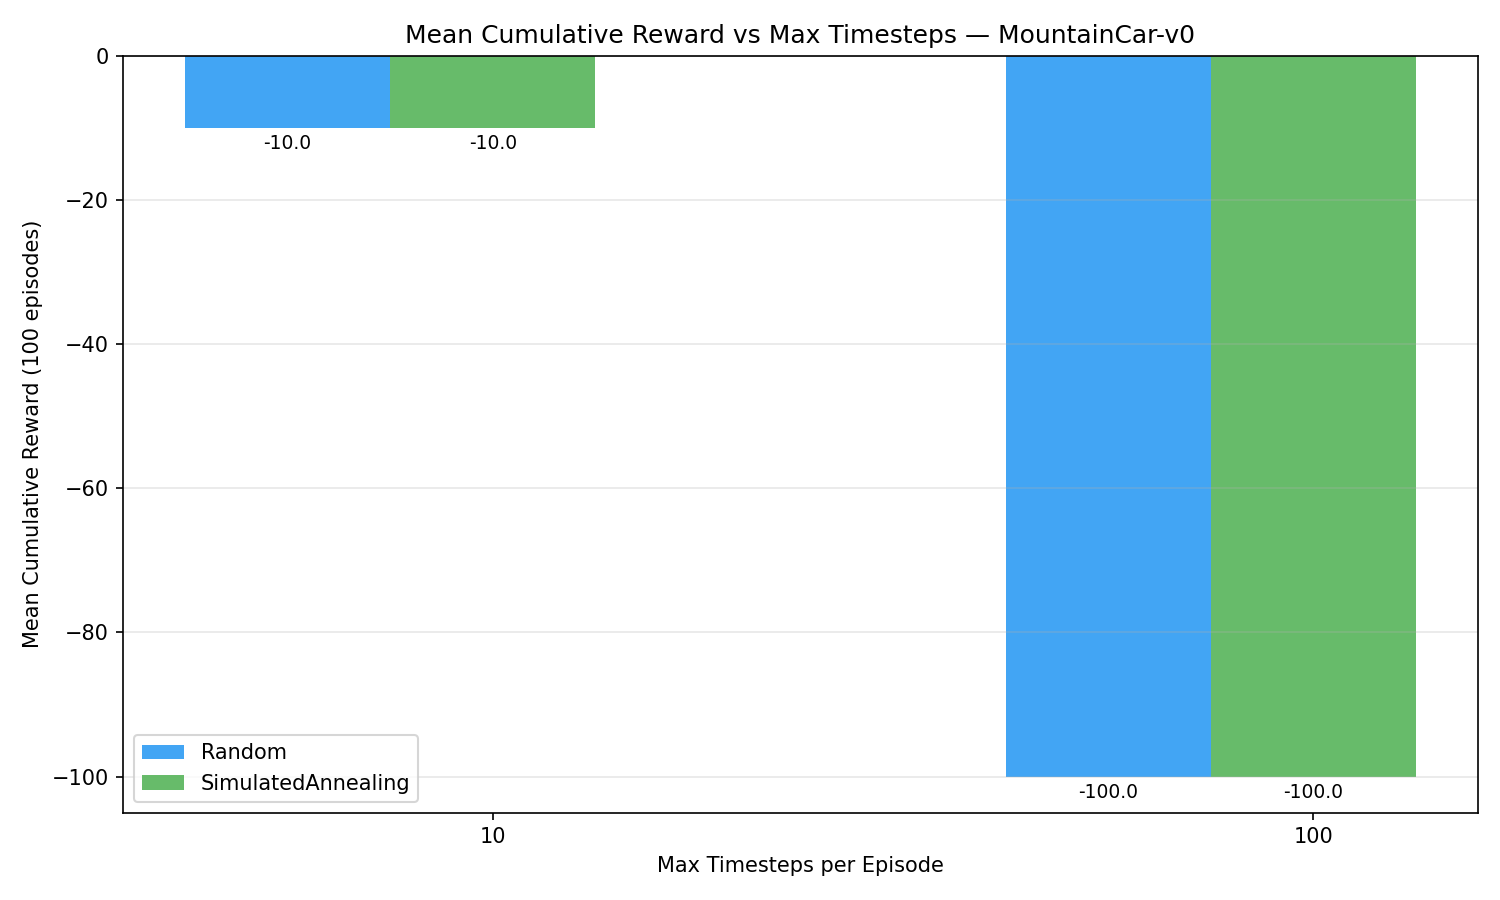
\includegraphics[width=0.85\textwidth]{exp1_MountainCar_v0.png}
    \caption{Μέση ανταμοιβή (100 επεισόδια) για το MountainCar-v0.}
\end{figure}

\subsection{Πείραμα 2: Καμπύλη Μάθησης (Non-Stationary)}
Παρατηρούμε την απόδοση σε 1000 επεισόδια ($max\_timesteps=100$).

\begin{figure}[h]
    \centering
    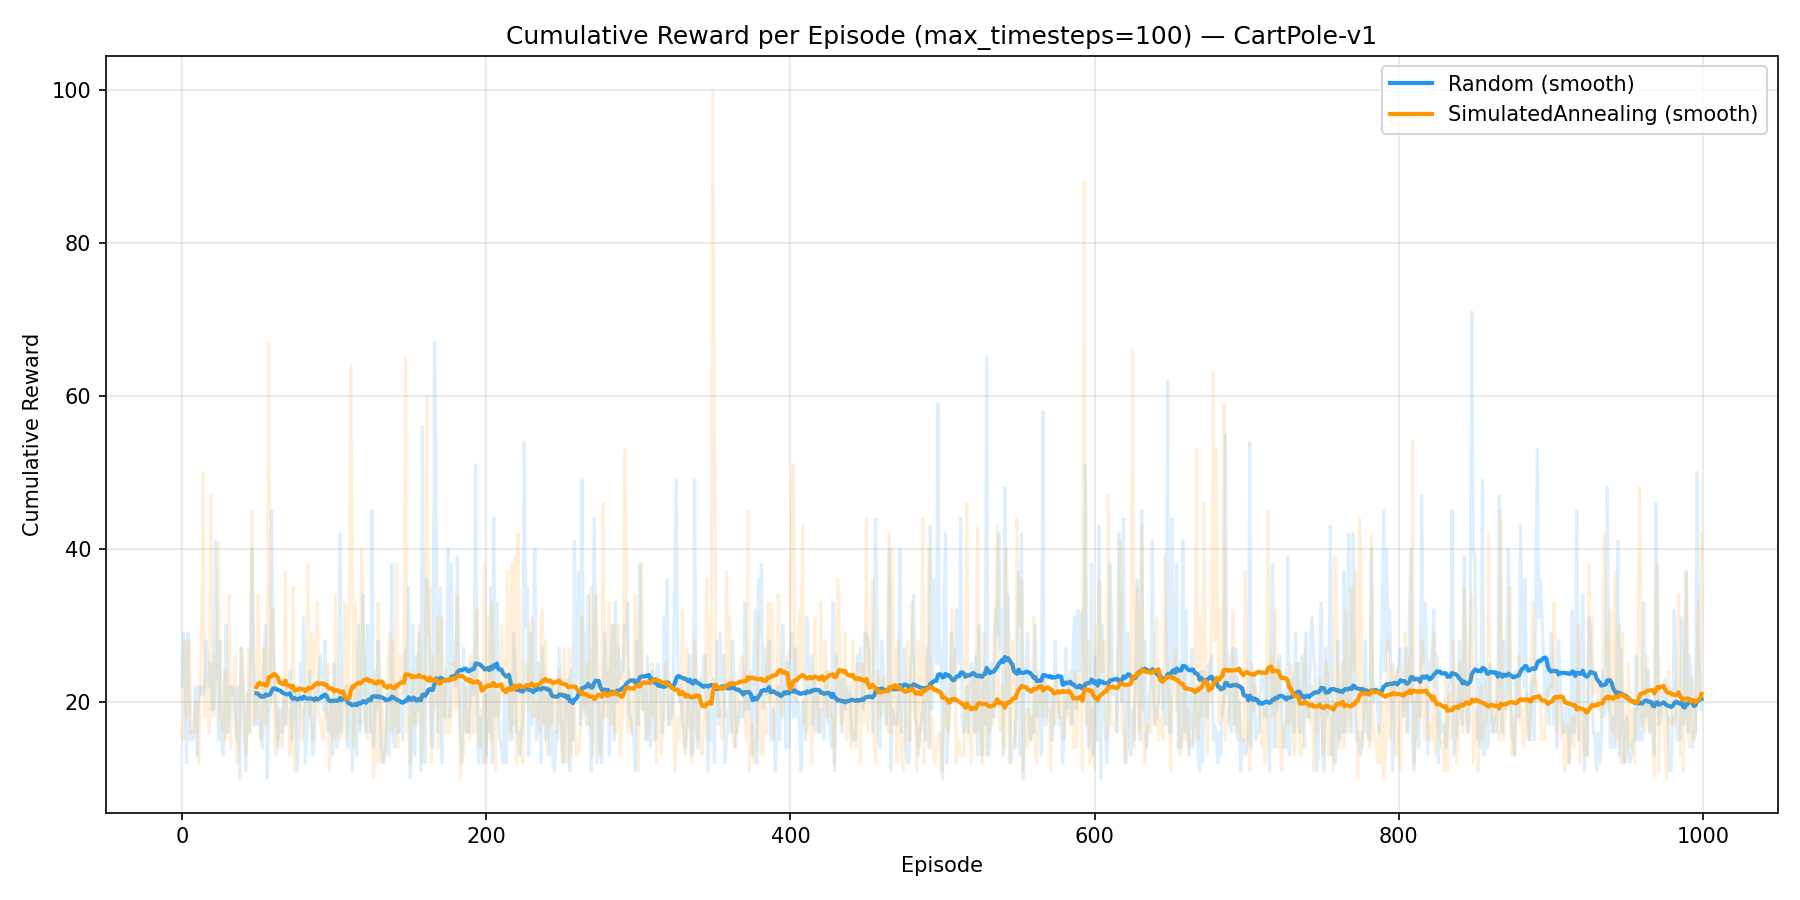
\includegraphics[width=0.85\textwidth]{exp2_CartPole_v1.png}
    \caption{Εξέλιξη συσσωρευμένης ανταμοιβής στο CartPole-v1 καθώς οι παράμετροι μεταβάλλονται.}
\end{figure}

\subsection{Θερμοκρασία Simulated Annealing}
\begin{figure}[h]
    \centering
    \includegraphics[width=0.7\textwidth]{sa_temperature_plot.png}
    \caption{Cooling schedule του Simulated Annealing πράκτορα.}
\end{figure}

\section{Συμπεράσματα}
Η ανάλυση των αποτελεσμάτων δείχνει ότι... [Συμπληρώστε με βάση τα δικά σας ευρήματα, π.χ. ο SA υπερέχει στο CartPole λόγω ευελιξίας, ενώ ο HC είναι ταχύτερος].

\end{document}
